%-------------------------------------------------
% FileName: main.tex
% Author: Safin (zhaoqid@zsc.edu.cn)
% Version: 0.1
% Date: 2020-05-12
% Description: 主文档,包含其它tex文档
%     如果要增加新的章节,请先到 tex目录增加文件,再input
%     如果附录没有内容,就注释掉
% Others: 编译方法参考 make.sh
%         适配TeXLive2020
%         必须用 [UTF-8无BOM] 编码
% History: origin
%-------------------------------------------------

\documentclass{style/zscthesis} % 自定义thesis

% 在正式撰写论文之前,请移步
% https://gitee.com/yeyunxiaopan/zsc-cs-latex-thesis
% 把模板的使用教程简单浏览一下
% 也可以对照B站视频一起看
% https://www.bilibili.com/video/av328559652

% Latex模板撰写的论文最终输出成PDF文档,当然不可能和Word一模一样。
% 如果觉得表格编辑有点麻烦,可以使用[在线工具](https://www.tablesgenerator.com/)。
% 如果图片导致文中有大段空白,可以通过调整文字和图片的位置,以及设置正确的浮动方式,来抑制文中的大段空白。
% 切记,参考文献,一定要在文中引用,才能出现在最后的参考文献章节。
% 切记,图片和表格一定要在文中引用,千万不能写,如下图,如下表


\begin{document} 
    %-------------------------------------------------
% FileName: frontinfo.tex
% Author: Safin (zhaoqid@zsc.edu.cn)
% Version: 0.1
% Date: 2020-05-12
% Description: 封面
% Others: 
% History: origin
%------------------------------------------------- 

% 根据个人信息修改{}中的内容------------------------
% 论文题目
\mytitle{中山学院\LaTeX{}论文模板设计与实现} 
% 英文题目
\MYTITLE{Design and Implementation of \LaTeX{} Thesis of Zhongshan Institute}
% 教学指导单位 
\institute{计算机学院} 
% 专业名称 
\major{计算机科学与技术}  
% 学号 多个学号用~分隔,如果要分行用\\分隔
\studentid{2016030105007~~2016061302082~~2016061308888} 
% 学生姓名 多个学生用~分隔,如果要分行用\\分隔
\student{常鑫~朱婵~虚若无} 
% 指导教师(职称) 多个导师用~分隔,如果要分行用\\分隔
\advisor{邓招奇(讲师) ~~战清风(副教授)} 
% 指导单位 
% \institute{计算机学院} 
% 完成时间  
%\completedate{{\number\year}年5月16日}

% 以下不用改动-------------------------------------
% 加入书签, bm@frontpage要唯一
\currentpdfbookmark{\deffrontpage}{bm@frontpage}
% 封面无页眉页脚
\thispagestyle{empty}
% 根据以上的参数 生成标题页
\mymaketitle

       % 封面
    %%-------------------------------------------------
% FileName: declaration.tex
% Author: Safin (zhaoqid@zsc.edu.cn)
% Version: 0.1
% Date: 2021-01-24
% Description: 声明
% Others: 如无需要,不用修改本文件
% History: origin
%-------------------------------------------------

% 断页
\clearpage
% 加入书签, bm@declarationpage要唯一
\currentpdfbookmark{\defdeclarationpage}{bm@declarationpage}
% 封面无页眉页脚
\thispagestyle{empty}
\makedeclaration
     % 声明
    %-------------------------------------------------
% FileName: abstract-ch.tex
% Author: Safin (zhaoqid@zsc.edu.cn)
% Version: 0.1
% Date: 2020-05-12
% Description: 中文摘要
% Others: 
% History: origin
%------------------------------------------------- 

% 以下不用改动-------------------------------------
% 断页
\clearpage
% 页码从1开始计数
\setcounter{page}{1}
% 大写罗马数字显示页码
\pagenumbering{Roman}
% 加入书签, bm@abstractname要唯一
\currentpdfbookmark{\defabstractname}{bm@abstractname}
% \chapter*{} 表示不编号,不生成目录
% \markboth{}{} 用于页眉
% 此处以中文题目作为章题目
%\chapter*{\centering{\deftitle}}


\markboth{\defabstractname}{}

%专业一行



%学生老师一行
\begin{center}
    {\zihao{3}\heiti {\deftitle}} \\
    \vspace*{1em}
    {\defmajor} \ 专业
    \\
    %空一行
    \vspace*{1em}
    学生:{\defstudent} 指导老师:{\defadvisor}
\end{center}

% 修改摘要和关键词---------------------------------
% 中文摘要

\abstract{
    qDou---豆瓣Symbian客户端,采用的是Qt进行编写。豆瓣是一家Web2.0网站,豆瓣主要通过用户点击及购买电子商务网站的相关产品,来获得收入。
    本次设计的qDou将主要是采用Qt的Graphics View框架编写,部分框架运用Declarative UI(Qt的下一代控件),在与豆瓣官方数据接口的交换上,利用豆瓣提供的Api key,通过OAuth协议进行对豆瓣数据的访问,修改以及提交。
    利用豆瓣网提供的API结合Qt的下一代控件Declarative UI 轻松的实现了具有平滑,收放自如, 动态变换的一款豆瓣客户端,这种控件主要针对于移动平台上,比如手机或者上网本。采用Qml语言使开发者和设计者在完成他们工作的时候更多的高效。另一方面这种简单易学的语言,是那些不熟悉C++的开发人员可以方便的使用Qt。为了保护豆瓣用户私有数据的安全,豆瓣采用OAuth协议来完成数据的写入,修改和删除。
    S60下豆瓣客户端新增了如搜索书籍,电影,音乐查询,收发豆邮等更强大的功能,同时你可以读取他们的评论,看看其他豆瓣的用户对这个条目时什么观点或者推荐好的条目给你的好友。另一方面,qdou 提供了朋友之间的数据可视化,通过豆瓣这个巨大的网络,你可以发现你与其他人之间的联系,共同的爱好.这些功能满足了时下网络社交生活的需要,更增加了无穷乐趣。由于使用Qt进行开发,所以qDou可以轻松的发布到Symbian Maemo,webOs,甚至Android上。
    
}

% 中文关键词 空格:\ (反斜杠后跟空格)  使用命令~
% 关键词是供检索用的主题词条,应采用能覆盖毕业设计(论文)主要内容的通用技术词条(参照相应的技术术语标准)。关键词一般为3~5个,每个关键词不超过5个字。
\keywords{毕业设计 \ 作品 \ 技术\ 结果;意义}


     % 中文摘要
    %-------------------------------------------------
% FileName: abstract-en.tex
% Author: Safin (zhaoqid@zsc.edu.cn)
% Version: 0.1
% Date: 2020-05-12
% Description: 英文摘要
% Others: 
% History: origin
%------------------------------------------------- 

% 以下不用改动-------------------------------------
% 断页
\clearpage
% 加入书签, bm@ABSTRACTNAME要唯一
\currentpdfbookmark{\defABSTRACTNAME}{bm@ABSTRACTNAME}
% \chapter*{} 表示不编号,不生成目录
% \markboth{}{} 用于页眉
% 此处以英文题目作为章题目
%\chapter*{\defTITLE \markboth{\defABSTRACTNAME}{}}
\chapter*{\markboth{\defABSTRACTNAME}{}}


\begin{center}
    {\zihao{3}\heiti{\defTITLE}}
\end{center}
\vspace*{1em}
% 修改摘要和关键词---------------------------------
% 英文摘要
% 英文摘要与中文摘要的内容应一致。
\ABSTRACT{
Fourscore and seven years ago, our fathers brought forth upon this continent a new Nation, conceived in Liberty, and dedicated to the proposition that all men are created equal. Now, we are engaged in a great Civil War, testing whether that Nation, or any nation so conceived and so dedicated, can long endure. We are met on a great battlefield of that war. We have come to dedicate a portion of that field as a final resting-place for those who here gave their lives that that Nation might live. It is altogether fitting and proper that we should do this.

But, in a larger sense, we cannot dedicate, we cannot consecrate, we cannot hallow this ground. The brave men, living and dead, who struggled here, have consecrated it far above our poor power to add or detract. The world will little note nor long remember what we say here, but it can never forget what they did here. It is for us, the living, rather to be dedicated here to the unfinished work which they who fought here have thus far so nobly advanced. It is rather for us to be here dedicated to the great task remaining before us; that from these honored dead, we take increased devotion to that cause for which they gave the last full measure of devotion; that we here highly resolve that these dead shall not have died in vain, that this Nation, under GOD, shall have a new birth of freedom; and that government of the People by the People and for the People shall not perish from the earth.
}

% 英文关键词
% 每一个英文关键词都必须与中文关键词一一对应。
\KEYWORDS{Thesis; Hello world; Good luck; Congratulations}




 

     % 英文摘要
    %-------------------------------------------------
% FileName: content.tex
% Author: Safin (zhaoqid@zsc.edu.cn)
% Version: 0.1
% Date: 2020-05-12
% Description: 目录
% Others: 如无需要,不用修改本文件
% History: origin
%-------------------------------------------------

% 断页
\clearpage
% 加入书签, bm@contentsname要唯一
\currentpdfbookmark{\contentsname}{bm@contentsname}
% 生成目录

    \renewcommand{\contentsname}{\centering 目\hspace{1em}录 \par}


\tableofcontents 

% 断页
\clearpage
% 加入书签, bm@listfigurename要唯一
\currentpdfbookmark{\listfigurename}{bm@listfigurename}
% 生成图目录
%\listoffigures
{
% 很弱智的,为每个图目录前加上 "图"
\let\oldnumberline\numberline
\renewcommand{\numberline}{\figurename~\oldnumberline}
\listoffigures
}


% 断页
\clearpage
% 加入书签, bm@listtablename要唯一
\currentpdfbookmark{\listtablename}{bm@listtablename}
% 生成表目录
% \listoftables
{
% 很弱智的,为每个表目录前加上 "表"
\let\oldnumberline\numberline
\renewcommand{\numberline}{\tablename~\oldnumberline}
\listoftables
}


         % 目录 (如无需要,不用修改)
    %-------------------------------------------------
% FileName: chapt-1.tex
% Author: Safin (zhaoqid@zsc.edu.cn)
% Version: 0.1
% Date: 2020-05-12
% Description: 第1章
% Others: 
% History: origin
%------------------------------------------------- 

% 断页
\clearpage
% 页码从1开始计数
\setcounter{page}{1} 
% 阿拉伯数字显示页码
\pagenumbering{arabic}

\chapter{绪论}

\section{课题背景}
简要介绍本文的开发背景。明确说明哪些是别人已经做过的工作,哪些是自己要做的工作。


% 分段是通过空行来实现的
话说得远一点,正是因为很多人不接受休谟的这个观点,才使得文艺创作者们有各种花招可以玩。比如《黑客帝国》后两集里的招数:让观众怀疑反抗军的基地也是虚拟出来的。比如《盗梦空间》里,让观众怀疑所谓的真实世界还是一个梦境。

% 引用参考文献 [1]
叔本华认为,我们可以提高自己对这世界的认识(当然是去认识叔本华所理解的那个世界),把自己的感情和欲望上升为全人类的感情和欲望,这样就可以消除个人的欲望\cite{chen2005laser}。

% 引用多篇参考文献 [1-3]
贪婪是人的本性,也是资本主义社会发展的必不可少的动力。但是今天的资本主义社会学会了用很多方法去克制个人贪欲。比如通过宗教的约束,比如通过立法的形式,遏制垄断企业(可怜的微软),遏制不正当和不道德的竞争,给工人更多的福利\cite{chen2005laser, mittelbach2004latex, zhen2018leave}。

% 下面是一个有序列表的例子,默认编号
别人已经研究的工作包括:
\begin{enumerate}
	\item 古希腊的斯多葛学派就相信部分决定论。他们认为我们不能控制事物,但是可以控制我们自己对待生活的方式。所以这个学派提倡随遇而安的生活态度\cite{zhou2002nerualnet}。
	\item 斯宾诺莎是用类似于几何的逻辑一步步推出整个哲学体系的。这意味着,他相信世间万物之间都有着严格的逻辑关系。这必然也会导致决定论\cite{qi2020deeplearning}。
	\item 休谟认为他之前的经验主义者和理性主义者都存在根本缺陷。休谟的回答是,不知道就不知道,没关系。我们能得到的经验就是面前的生活,在有明确的证据证明面前的生活都是幻觉之前,我们就照着自己平时的经验正常生活下去就可以了。我们没必要也没能力去无限地怀疑世界\cite{partl2019short}。
\end{enumerate}

% 有序列表嵌套 定制编号
唐诗,宋词,元曲举例:
\begin{enumerate}
	\item 唐诗
	\begin{enumerate} 
		\item 蜀道难(李白)噫吁嚱,危乎高哉!蜀道之难,难于上青天!蚕丛及鱼凫,开国何茫然!尔来四万八千岁,不与秦塞通人烟。西当太白有鸟道,可以横绝峨眉巅。地崩山摧壮士死,然后天梯石栈相钩连。上有六龙回日之高标,下有冲波逆折之回川。黄鹤之飞尚不得过,猿猱欲度愁攀援。青泥何盘盘,百步九折萦岩峦。扪参历井仰胁息,以手抚膺坐长叹。
		\item 春晓(孟浩然)春眠不觉晓,处处闻啼鸟。夜来风雨声,花落知多少。
	\end{enumerate}
	\item 宋词
	\begin{enumerate}
		\item 破阵子(辛弃疾)醉里挑灯看剑,梦回吹角连营。八百里分麾下炙,五十弦翻塞外声,沙场秋点兵。马作的卢飞快,弓如霹雳弦惊。了却君王天下事,赢得生前身后名。可怜白发生!
		\item 赤壁怀古(苏轼)大江东去,浪淘尽,千古风流人物。故垒西边,人道是,三国周郎赤壁。乱石穿空,惊涛拍岸,卷起千堆雪。江山如画,一时多少豪杰。遥想公瑾当年,小乔初嫁了,雄姿英发。羽扇纶巾,谈笑间,樯橹灰飞烟灭。故国神游,多情应笑我,早生华发。人生如梦,一尊还酹江月。
	\end{enumerate}
	\item 元曲
	\begin{enumerate}
		\item 窦娥冤(关汉卿)花有重开日,人无再少年。不须长富贵,安乐是神仙。老身蔡婆婆是也。楚州人氏,嫡亲三口儿家属。不幸夫主亡逝已过,止有一个孩儿,年长八岁。俺娘儿两个,过其日月。家中颇有些钱财。这里一个窦秀才,从去年问我借了二十两银子,如今本利该银四十两。我数次索取,那窦秀才只说贫难,没得还我。他有一个女儿,今年七岁,生得可喜,长得可爱。我有心看上他,与我家做个媳妇,就准了这四十两银子,岂不两得其便!他说今日好日辰,亲送女儿到我家来。老身且不索钱去,专在家中等候。这早晚窦秀才敢待来也。
		\item 秋思(马致远)枯藤老树昏鸦,小桥流水人家,古道西风瘦马。夕阳西下,断肠人在天涯。
	\end{enumerate}
\end{enumerate}

\section{目的意义}
介绍本课题的研究意义、研究目的、主要研究内容、研究范围和应该解决的问题。

% 下面演示怎么增加子标题
\subsection{目的意义1}
\subsubsection{目的意义11}
\subsubsection{目的意义12}
\subsubsection{目的意义13}
\subsection{目的意义2}
\subsection{目的意义3}
\subsection{目的意义4}

\section{论文主要工作}
介绍本研究课题的来源及主要研究内容。

本作品分工如下,虚若无同学实现:
% 下面是一个无序列表的例子
\begin{itemize}
	\item 系统架构设计;
	\item 功能模块的设计与实现;
	\item web端的编程与实现;
	\item 数据库设计。
\end{itemize}

欧阳潇潇同学实现:
\begin{itemize}
	\item 微信小程序的设计与实现;
	\item 微信端接口的实现;
	\item 数据库设计。
\end{itemize}

\section{论文组织结构}

第1章介绍了考研教室预约系统的课题背景,目的意义,组员分工,全文的组织结构。

第2章介绍了系统开发所涉及的相关技术。包括MySQl数据库,前后端分离。Spring Boot,Ajax,微信小程序开发。
 
第3章对考研教室预约系统做了详细的需求分析,详细介绍了系统在实际应
用中的功能需求,系统的业务分析,系统的用例分析,系统的功能分析和非功能性需求。

第4章考研教室预约系统的系统总体设计,详细介绍了系统的总体结构和系统模块的设计以及数据库的设计和E-R图。

第5章考研教室预约系统的系统的实现,介绍了系统实现的关键技术,以及WEB端和移动端各个功能模块的实现。

第6章总结和展望,总结了系统的开发工作,分析了系统目前存在的问题及系统需要进一步完善的地方。          % 第1章
    %-------------------------------------------------
% FileName: chapt-2.tex
% Author: Safin (zhaoqid@zsc.edu.cn)
% Version: 0.1
% Date: 2020-05-12
% Description: 第2章
% Others: 
% History: origin
%------------------------------------------------- 

% 断页
% \clearpage
\chapter{相关技术和理论基础}

\section{技术与理论基础}
介绍在系统的开发过程中所要用到的技术\cite{timmurphy}以及与系统相关的理论知识\cite{huwei2017latex2e}。

\section{质能方程}
% 行内公式,用两个$
质能方程即描述质量与能量之间的当量关系的方程\cite{liuxiaopingwordandtex}。质能方程$e=mc^2$,$e$表示能量,$m$代表质量,而$c$则表示光速,由爱因斯坦提出\cite{yassin1994latex}。

\section{牛顿力学}
% 下面说明公式的引用。
任何物体都要保持匀速直线运动或静止状态\cite{liu2013latex},直到外力迫使它改变运动状态为止,见公式\eqref{eq:newton}。
% 行间公式,用环境 equation
% \label用于标注公式,在别处引用
\begin{equation}\label{eq:newton}
	\vec{F}=m\vec{a} 
\end{equation}

\section{勾股定理}
勾股定理是一个基本的几何定理,指直角三角形的两条直角边的平方和等于斜边的平方,如方程\eqref{eq:pythagoraslaw}所示。中国古代称直角三角形为勾股形,并且直角边中较小者为勾,另一长直角边为股,斜边为弦,所以称这个定理为勾股定理,也有人称商高定理\cite{he2017mask}。
\begin{equation}\label{eq:pythagoraslaw}
    a^2 + b^2 = c^2  
\end{equation}

\section{线性代数}
线性代数是数学的一个分支,它的研究对象是向量,向量空间(或称线性空间),线性变换和有限维的线性方程组。向量空间及其线性变换,以及与此相联系的矩阵(形如\eqref{eq:linearalgebra})理论,构成了线性代数的中心内容。
\begin{equation}\label{eq:linearalgebra}
	\begin{pmatrix}
		a_{11} & a_{12} & a_{13}\\ 
		a_{21} & a_{22} & a_{23}\\  
		a_{31} & a_{32} & a_{33}   
	\end{pmatrix}  
\end{equation}

\section{量子力学}
对于微观粒子的运动,可以用薛定谔方程来描述,
\begin{equation}
	\hat H \Psi = i \hbar \frac{\partial \Psi}{\partial t}
\end{equation}
其中$\hat H $为哈密顿算符,一般的从一个粒子的质量与这个粒子的势能函数,就可以得到这个方程,然后再根据给定的初值条件和边值条件,就可以解出我们需要的描述粒子运动状态的波函数来,然后波函数的绝对值平方就给出了粒子在一定时空位置的分布几率,这就是我们所能得到的关于粒子的最详尽的运动状态信息。


    %-------------------------------------------------
% FileName: chapt-3.tex
% Author: Safin (zhaoqid@zsc.edu.cn)
% Version: 0.1
% Date: 2020-05-12
% Description: 第3章
% Others: 
% History: origin
%------------------------------------------------- 

% 断页
% \clearpage 

\chapter{系统分析(需求分析)}

\section{功能需求分析}
% 引用图片的例子
描述系统的功能性需求,可以通过数据流图或UML的用例图等图表工具来部来定义系统的功能需求,并把需求和设计完全分离开。如图\ref{fig:single}所示。

% xelatex 支持的图片格式
% 矢量图 .pdf .eps 
% 位图 .jpg .png .bmp

% figure环境
% [H] 浮动优先级,当前位置,但尺寸过大的浮动体可能使得分页比较困难

% [htbp!] 浮动方式 请参考一份(不太)简短的 LATEX 2" 介绍,3.9节
% h 当前位置(代码所处的上下文)
% t 顶部
% b 底部
% p 单独成页
% ! 在决定位置时忽视限制
% 排版位置的选取与参数里符号的顺序无关, 
% LATEX 总是以 h-t-b-p 的优先级顺序决定浮动体位置。
% 也就是说 [!htp] 和 [ph!t] 没有区别。

\begin{figure}[H]
	% 居中
	\centering 
	% width=.5\textwidth 文档宽度的0.5
	% fig1图片放在img目录下,在此处引用无需img/前缀和图片格式后缀(png, jpg等)
	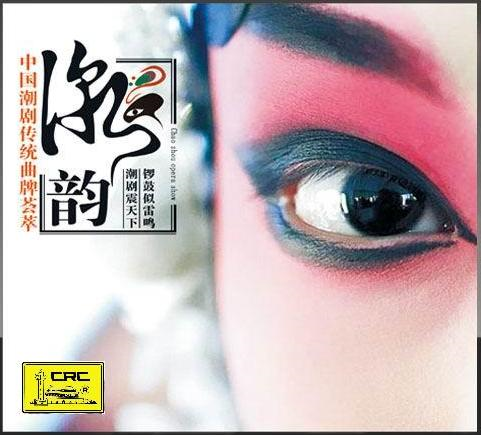
\includegraphics[width=.5\textwidth]{fig1} 
	% label紧接caption之后,用于引用
	\caption{这是一个很长很长的图的名字图的名字图的名字图的名字图的名字图的名字图的名字图的名字图的名字图的名字图的名字图的名字图的名字图的名字图的名字图的名字图的名字图的名字图的名字图的名字图的名字图的名字图的名字图的名字图的名字图的名字图的名字图的名字图的名字图的名字图的名字图的名字图的名字图的名字图的名字}
	\label{fig:single}
\end{figure}


\section{系统业务分析}
如图\ref{fig:double}所示。

% 两个图并排
\begin{figure}[H]
	\centering
    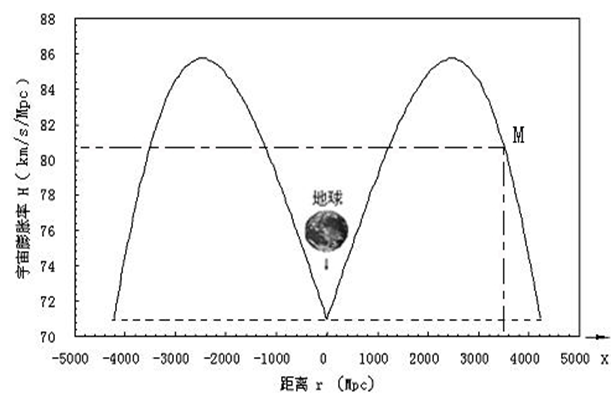
\includegraphics[width=.4\textwidth]{fig2}
    \quad % 横向两图的间距
    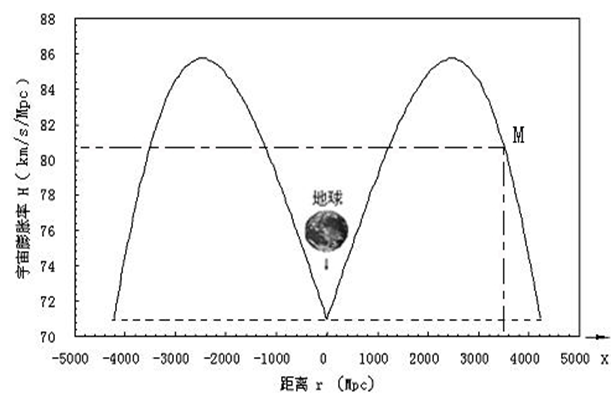
\includegraphics[width=.4\textwidth]{fig2} 
	\caption{两个图}
	\label{fig:double}
\end{figure}

\section{系统用例分析}

如图\ref{fig:fourimg}所示。

% 四个图并排
\begin{figure}[H]
	\centering
    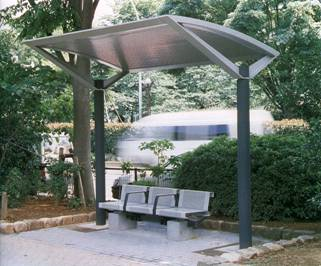
\includegraphics[width=.4\textwidth]{fig3}
    \quad 
	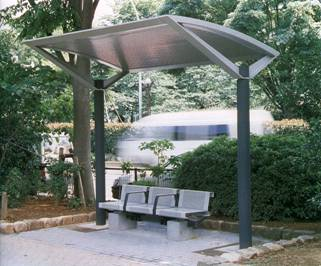
\includegraphics[width=.4\textwidth]{fig3} 
	% 空一行,分两行排版

	% 垂直间距 ex当前字号下小写字母 x 的高度
	\vspace{1ex} 
	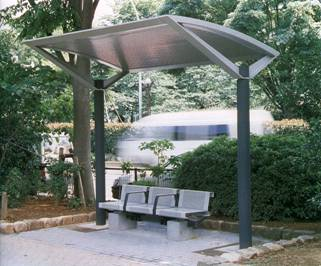
\includegraphics[width=.4\textwidth]{fig3}
	\quad
	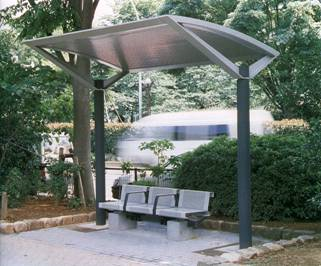
\includegraphics[width=.4\textwidth]{fig3}
	\caption{四个图}
	\label{fig:fourimg}
\end{figure}

\section{系统功能分析}

% % tikz绘图
% % 参考文档 texdoc tikz

% \begin{figure}[H]
% 	\centering
% 	\begin{tikzpicture}
% 		\begin{scope}[canvas is zy plane at x=0]
% 		\draw (0,0) circle (1cm);
% 		\draw (-1,0) -- (1,0) (0,-1) -- (0,1);
% 		\end{scope}
% 		\begin{scope}[canvas is zx plane at y=0]
% 		\draw (0,0) circle (1cm);
% 		\draw (-1,0) -- (1,0) (0,-1) -- (0,1);
% 		\end{scope}
% 		\begin{scope}[canvas is xy plane at z=0]
% 		\draw (0,0) circle (1cm);
% 		\draw (-1,0) -- (1,0) (0,-1) -- (0,1);
% 		\end{scope}
% 	\end{tikzpicture}
% 	\caption{画个圈圈}\label{fig:tikzcircle}
% \end{figure}

% \begin{figure}[H]
% 	\centering
% 	\begin{tikzpicture} 
% 		\draw[-stealth,line width=0.2pt] (-0.5,0) -- (4.5,0);
% 		\draw[-stealth,line width=0.2pt] (0,-0.5) -- (0,2.5);
% 		\coordinate (a) at (0.5,1.9);
% 		\coordinate (b) at (4,1.2);
% 		\node[below] (a0) at (a |- 0,0) {$a$};
% 		\node[below] (b0) at (b |- 0,0) {$b$};
% 		\filldraw[fill=gray!20,draw,thick]
% 		(a0) -- (a) .. controls (1,2.8) and (2.7,0.4) .. (b) -- (b0) -- cycle;
% 		\node[above right,outer sep=0.2cm, rounded corners,
% 		fill=green!20,draw=gray,text=blue!60!black,scale=0.6]
% 		at (b) {$\displaystyle \int_a^b {f(x)\,\mathrm{d}x} = F(b) - F(a)$}; 
% 	\end{tikzpicture}
% 	\caption{画个曲线}\label{fig:tikzcurve}
% \end{figure}


% \begin{figure}[H]
% 	\centering
% 	\tikz \graph [tree layout, nodes={draw,circle}, sibling sep=0pt]{ r -> { a, , ,b -> {c,d}, ,e} };
% 	\caption{画个树}\label{fig:tikztree}
% \end{figure}


\section{非功能需求分析}
描述系统的一些非功能方面的需求,如开发和运行环境、性能、人机交互、用户体验等。
 
 


           % 增加新章节到tex目录,此处input
    %-------------------------------------------------
% FileName: chapt-4.tex
% Author: Safin (zhaoqid@zsc.edu.cn)
% Version: 0.1
% Date: 2020-05-12
% Description: 第4章
% Others: 
% History: origin
%------------------------------------------------- 


% 断页
% \clearpage
\chapter{系统设计}

\section{总体设计}
描述根据系统的需求分析,确定系统的功能模块构成。

\section{详细设计}
说明各个功能模块的数据结构和实现算法。


C源代码
\begin{clan}
    #include <stdio.h>  
    int main()                  //main 入口函数  
    {  
        printf("Hello,World!"); //printf 函数打印  
        return 1;               //函数返回值  
    }   
\end{clan}


matlab源代码
    \begin{matlab}
    function F=random()
    a=[1 2];
    Prob=[0.99 0.01];
    F=randsrc(1,1,[a;Prob]);

    areas=[]
    for i=1:100
    x=unifrnd(0,10,[1,100]);
    y=unifrnd(0,10,[1,100]);
    frequency=sum(x<=1)+sum(y<=1);
    area=100*frequency/100;
    areas=[areas,area];
    end
\end{matlab}


python源代码
\begin{python}
    from multiprocessing import Pool
    import os, time, random

    def long_time_task(name):
        print('Run task %s (%s)...' % (name, os.getpid()))
        start = time.time()
        time.sleep(random.random() * 3)
        end = time.time()
        print('Task %s runs %0.2f seconds.' % (name, (end - start)))

    if __name__=='__main__':
        print('Parent process %s.' % os.getpid())
        p = Pool(4)
        for i in range(5):
        p.apply_async(long_time_task, args=(i,))
        print('Waiting for all subprocesses done...')
        p.close()
        p.join()
        print('All subprocesses done.')
\end{python}




C++源代码
\begin{cpp}
    #include <iostream>               //std::cout 要用到的头文件  
    #include <stdio.h>                //标准输入输出头文件  

    int main()  
    {  
        printf("Hello,World!--Way 1\n");    //printf 语句打印  
        puts("Hello,World!--Way 2");        //puts 语句  
        puts("Hello," " " "World!--Way 3"); //字符串拼接  
        std::cout << "Hello,World!--Way 4" << std::endl; //C++ 教科书上写法  
        return 1;                                        //作为注释  
    }  
\end{cpp}




Csharp源代码
\begin{clan}
    //FileName: HelloWorld.cs  
    using System;  
    class TestApp  
    {  
        public static void Main()  
        {  
            Console.WriteLine("Hello,World!");  
            Console.ReadKey();  
        }  
    }   
\end{clan}

java源代码
\begin{java}
    #FileName: HelloWorld.java 
    #如果有 public 类的话,类名必须和文件同名,注意大小写   
    public class HelloWorld   
    {  
        #Java 入口程序,程序从此入口  
        public static void main(String[] args)  
        {  
            #向控制台打印一条语句  
            System.out.println("Hello,World!");  
        }  
    }  
\end{java}


js源代码
\begin{javascript}
    var sys = require("sys");    #导入需要的 sys 模块  
    sys.puts("Hello,World!");    #调用里面的 puts 函数来打印字符串  
\end{javascript}

php源代码
\begin{php} 
    <?php  
        echo "Hello,World!";            //打印语句  
        echo "The first php program!";  //打印语句  
        echo phpinfo();                 //phpinfo()系统函数,输出环境信息  
    ?>    
\end{php}


go源代码
\begin{gogo}

    //filename: hello.go
    package main 
    import (
        "fmt"
        "os"
    )
    func main(){ //这个 { 不能另起一行
        fmt.Println("hello world!")
    }
\end{gogo}

html源代码
\begin{html}
    <!DOCTYPE html>  
    <html>  
        <body>  
            <h1>This is the first program!</h1>  
            <p>Hello,World!</p>  
        </body>  
    </html>
\end{html}

xml源代码 
\begin{xml}
    <?xml version="1.0"?>
    <class name="Student" table="student">
        <id name="id" column="id" ></id>
        <property name="name" column="name" ></property>
        <property name="age" column="age" ></property>
    </class> 
\end{xml}

sql源代码 
\begin{sql}
    SQL> CREATE TABLE MESSAGE (TEXT CHAR(15));            #创建表  
    INSERT INTO MESSAGE (TEXT) VALUES ('Hello, world!');  #插入表  
    SELECT TEXT FROM MESSAGE;                             #查询表  
    DROP TABLE MESSAGE;                                   #删除表               
    Table created.   
\end{sql}

tex源代码 
\begin{tex}
    \begin{figure}[H]
        % 居中
        \centering 
        % width=.5\textwidth 文档宽度的0.5
        % fig1图片放在img目录下,在此处引用无需img/前缀和图片格式后缀(png, jpg等)
        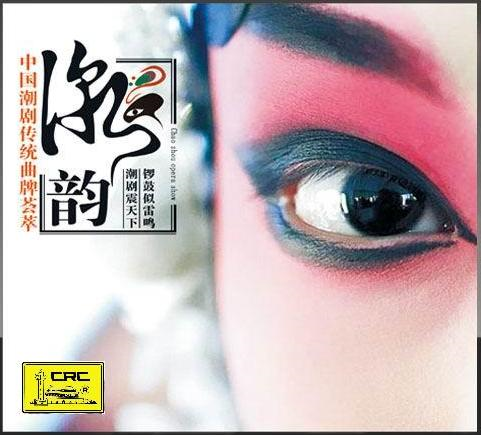
\includegraphics[width=.5\textwidth]{fig1} 
        % label紧接caption之后,用于引用
        \caption{这是一个图}
        \label{fig:single}
    \end{figure}
\end{tex} 
    %-------------------------------------------------
% FileName: chapt-5.tex
% Author: Safin (zhaoqid@zsc.edu.cn)
% Version: 0.1
% Date: 2020-05-12
% Description: 第5章
% Others: 
% History: origin
%------------------------------------------------- 


% 断页
% \clearpage
\chapter{系统实现与测试}

\section{系统实现}
介绍主要功能模块的编程实现以及系统的部署方法。

\section{系统测试}
阐述系统的测试技术、测试过程和测试结果。


% table环境
% [H] 浮动优先级,当前位置,但尺寸过大的浮动体可能使得分页比较困难

% [htbp!] 浮动方式 请参考一份(不太)简短的 LATEX 2" 介绍,3.9节
% h 当前位置(代码所处的上下文)
% t 顶部
% b 底部
% p 单独成页
% ! 在决定位置时忽视限制
% 排版位置的选取与参数里符号的顺序无关, 
% LATEX 总是以 h-t-b-p 的优先级顺序决定浮动体位置。
% 也就是说 [!htp] 和 [ph!t] 没有区别。

完全手动完成的表格,如表\ref{tab:tab1}所示。 % 通过label引用表格
\begin{table}[H] % H浮动优先级,当前位置
        \zihao{5} % 字号5
    \centering  % 居中
    \caption{一个表格}  % 表格标题
    \label{tab:tab1}  % 用于在正文中引用的label
    % 字母的个数对应列数,| 代表分割线
    % l代表左对齐,c代表居中,r代表右对齐
    \begin{tabular}{|c|c|c|c|}   
        \hline  % 表格的横线 
        1 & 2 & 3 & 4 \\  % 表格中的内容,用&分开,\\表示下一行
        \hline 
        0.1 & 0.2 & 0.3 & 0.4 \\
        \hline
    \end{tabular}
\end{table}

以下编辑器(TexStudio)的表格向导生成的表格,如表\ref{tab:tab2}所示。% 通过label引用表格
\begin{table}[H] % H浮动优先级,当前位置
        \zihao{5} % 字号5
	\centering  % 居中
	\caption{诗词曲} % 表格标题  
    \label{tab:tab2}   % 用于在正文中引用的label
    % 字母的个数对应列数,| 代表分割线
    % l代表左对齐,c代表居中,r代表右对齐
    \begin{tabular}{|c|c|c|c|}
        \hline  % 表格的横线 
          & 唐诗 & 宋词 & 元曲 \\ 
        \hline 
        1 & 李白 & 苏轼 & 关汉卿 \\ 
        \hline 
        2 & 白居易 & 辛弃疾 & 马致远 \\ 
        \hline 
        3 & 杜甫 & 李清照 & 张可久 \\ 
        \hline 
        4 & 王维 & 陆游 & 张养浩 \\ 
        \hline 
        5 & 孟浩然 & 欧阳修 & 徐再思 \\ 
        \hline 
    \end{tabular}  
\end{table}

嵌套表格,如表\ref{tab:tab3}所示。% 通过label引用表格
\begin{table}[H] % H浮动优先级,当前位置
        \zihao{5} % 字号5
	\centering  % 居中
	\caption{嵌套表格} % 表格标题  
    \label{tab:tab3}  % 用于在正文中引用的label
    % 字母的个数对应列数,| 代表分割线
    % l代表左对齐,c代表居中,r代表右对齐
    \begin{tabular}{|c|c|c|}
        \hline  % 表格的横线 
        a & b & c \\ \hline
        a & \multicolumn{1}{@{}c@{}|}
        {\begin{tabular}
{c|c}
            e & f \\ \hline
            e & f \\
        \end{tabular}}
        & c \\ \hline
        a & b & c \\ \hline
    \end{tabular}
\end{table}

控制列宽的表格,如表\ref{tab:tab4},表\ref{tab:tab5}所示。% 通过label引用表格
\begin{table}[H] % H浮动优先级,当前位置
    \zihao{5} % 字号5
    \centering  % 居中
    \caption{控制列宽的表格} % 表格标题  
    \label{tab:tab4}  % 用于在正文中引用的label 
    \begin{tabularx}{30em}  % 总列宽 30em
    % 多个 X 列格式平均分配列宽
        {|*{4}{>{\centering\arraybackslash}X|}}
        \hline  % 表格的横线 
        A & B & C & D \\ \hline
        a & b & c & d \\ \hline
    \end{tabularx}
\end{table}

\begin{table}[H] % H浮动优先级,当前位置
    \zihao{5} % 字号5
    \centering  % 居中
    \caption{诗词曲}  % 表格标题 
    \label{tab:tab5}  % 用于在正文中引用的label 
    % 总列宽 30em
    \begin{tabularx}{30em} 
    % 多个 X 列格式平均分配列宽
        {|*{4}{>{\centering\arraybackslash}X|}}
        \hline  % 表格的横线 
          & 唐诗 & 宋词 & 元曲 \\ 
        \hline 
        1 & 李白 & 苏轼 & 关汉卿 \\ 
        \hline 
        2 & 白居易 & 辛弃疾 & 马致远 \\ 
        \hline 
        3 & 杜甫 & 李清照 & 张可久 \\ 
        \hline 
        4 & 王维 & 陆游 & 张养浩 \\ 
        \hline 
        5 & 孟浩然 & 欧阳修 & 徐再思 \\ 
        \hline 
    \end{tabularx}  
\end{table}

控制行距的表格,如表\ref{tab:tab6}所示。% 通过label引用表格
\begin{table}[H] % H浮动优先级,当前位置
    \zihao{5} % 字号5
    \centering  % 居中
    \caption{控制行距的表格}  % 表格标题 
    \label{tab:tab6}  % 用于在正文中引用的label 
    \renewcommand\arraystretch{2.8} % 行距控制
    % 字母的个数对应列数,| 代表分割线
    % l代表左对齐,c代表居中,r代表右对齐
    \begin{tabular} {|c|c|c|c|}
        \hline % 表格的横线 
        A & B & C & D \\ \hline
        a & b & c & d \\ \hline
    \end{tabular}
\end{table}

表格单行内容太长,直接换行,如表\ref{tab:tab7},表\ref{tab:tab8}所示。% 通过label引用表格
\begin{table}[H] % H浮动优先级,当前位置
    \zihao{5} % 字号5
    \centering  % 居中
    \caption{单行内容太长直接换行}  % 表格标题 
    \label{tab:tab7}   % 用于在正文中引用的label
    % 字母的个数对应列数,| 代表分割线
    % l代表左对齐,c代表居中,r代表右对齐
    \begin{tabular}{|c|c|c|c|} 
        \hline  % 表格的横线 
          & 唐诗 & 宋词 & 元曲 \\ 
        \hline 
        1 & 李白李白李白 & 苏轼苏轼苏轼苏轼 & 关汉卿关汉卿关汉卿关汉卿 \\
         & 李白李白李白李白 & 苏苏轼苏轼轼 & 关汉卿关汉卿关汉卿 \\
        \hline 
        2 & 白居易 & 辛弃疾 & 马致远 \\ 
        \hline 
    \end{tabular}  
\end{table}


\begin{table}[H] % H浮动优先级,当前位置
    \zihao{5} % 字号5
    \centering  % 居中
    \caption{控制列宽单行内容太长直接换行}  % 表格标题 
    \label{tab:tab8}   % 用于在正文中引用的label 
    \begin{tabularx}{30em} % 总列宽 30em
    % 多个 X 列格式平均分配列宽
        {|*{4}{>{\centering\arraybackslash}X|}}
        \hline  % 表格的横线 
          & 唐诗 & 宋词 & 元曲 \\ 
        \hline 
        1 & 李白李白李白 & 苏轼苏轼苏轼苏轼 & 关汉卿关汉卿关汉卿关汉卿 \\
         & 李白李白李白李白 & 苏苏轼苏轼轼 & 关汉卿关汉卿关汉卿 \\
        \hline 
        2 & 白居易 & 辛弃疾 & 马致远 \\ 
        \hline 
    \end{tabularx}  
\end{table}

  
    %-------------------------------------------------
% FileName: chapt-6.tex
% Author: Safin (zhaoqid@zsc.edu.cn)
% Version: 0.1
% Date: 2020-05-12
% Description: 第6章
% Others: 
% History: origin
%------------------------------------------------- 

% 断页
% \clearpage
\addcontentsline{toc}{chapter}{总结级展望}

是对整个毕业设计工作的归纳和综合,对现有成果和尚存在的问题的描述,以及进一步开展研究的见解与建议。


 



% \begin{lstlisting}[language=TeX,frame=single,]
% { 
%   $\int f(x) \mathrm{d}x$
%   $\sum_{0}^{+\infty}$
%   \begin{center}
%   居中
%   \end{center}
% }
% \end{lstlisting}

          % 第6章
    %-------------------------------------------------
% FileName: reference.tex
% Author: Safin (zhaoqid@zsc.edu.cn)
% Version: 0.1
% Date: 2020-05-12
% Description: 参考文献
% Others: 如无需要,不用修改本文件
%         参考文献请到 bib/ref.bib中按格式增加
% History: origin
%-------------------------------------------------


% 参考文献是毕业设计(论文)不可缺少的组成部分,在毕业设计(论文)的撰写过程中应承认和尊重他人的知识成果,参考与引用的内容必须注明,杜绝抄袭、剽窃他人成果。同时,引用的资料应具有权威性,并对毕业设计(论文)有直接的参考价值。
% 要求查阅文献15篇(含)以上,其中外文文献3篇(含)以上,近三年公开发表的文献3篇(含)以上,书籍不超过5本,期刊([J])和论文集([C])8篇(含)以上,包括导师指定的全部参考文献。


% 断页
\clearpage

% hyperef 精确定位
% 设置一个anchor,主要针对\addcontentsline
% 防止目录,书签等指向错误位置 
\phantomsection

% 增加到目录,与chapter同级别
\addcontentsline{toc}{chapter}{\bibname}

%------------------------------------------
% 默认参考文献样式 plain
% \bibliographystyle{plain}
% gbt7714 顺序编码制
\bibliographystyle{bib/gbt7714-numerical} 
%------------------------------------------

% ref是BIBTEX数据库的文件名,不要带.bib 扩展名,实际文件 bib/ref.bib
\bibliography{bib/ref}




         % 参考文献 (修改bib/ref.bib)
    %-------------------------------------------------
% FileName: appendix.tex
% Author: Safin (zhaoqid@zsc.edu.cn)
% Version: 0.1
% Date: 2020-05-12
% Description: 附录
% Others: 如果没有内容,就在main.tex中注释掉
% History: origin
%------------------------------------------------- 


% 以下不用改动-------------------------------------
% 断页
% \clearpage



% hyperef 精确定位
% 设置一个anchor,主要针对\addcontentsline
% 防止目录,书签等指向错误位置 
% \phantomsection
% 增加到目录,与chapter同级别
% \addcontentsline{toc}{chapter}{\appendixname} 
% \chapter*{} 表示不编号,不生成目录
% \markboth 用于页眉
% \chapter*{\appendixname \markboth{\appendixname}{}} 

% appendix 用于附录章节的特殊编号 从A开始
\appendix

% 附录章
\chapter{算法} 

% 修改以下内容---------------------------------
对于一些不宜放入正文,又是毕业设计(论文)不可缺少的部分,或有重要参考价值的内容,可编入附录中。例如:过长的公式推导,大量的数据和图表,程序全文及其说明等。

\section{xxx} 

\section{cccc} 

\chapter{源码} 



\chapter{数据} 

        % 附录 (无内容请注释掉) 
    %-------------------------------------------------
% FileName: acknowledgement.tex
% Author: Safin (zhaoqid@zsc.edu.cn)
% Version: 0.1
% Date: 2020-05-12
% Description: 致谢
% Others: 
% History: origin
%------------------------------------------------- 

% 以下不用改动-------------------------------------
% 断页
\clearpage
% hyperef 精确定位
% 设置一个anchor,主要针对\addcontentsline
% 防止目录,书签等指向错误位置 
\phantomsection
%增加到目录,与chapter同级别
\addcontentsline{toc}{chapter}{\defacknowledgement}
% \chapter*{} 表示不编号,不生成目录
% \markboth{}{} 用于页眉
\chapter*{ \markboth{\defacknowledgement}{}}

%这里不知道怎么居中,就采用累加环境居中(可能描述有问题)
\begin{center}
    \centering{\defacknowledgement}
\end{center}


% 修改{}中的内容---------------------------------
\acknowledgement{

简述自己通过毕业设计(论文)的体会,向给予指导、合作、支持及协助完成研究工作的单位、组织或个人致谢。致谢的文字虽不多,却是论文不可缺少的内容。内容应简洁明了、实事求是,避免俗套。

第二段致谢。

第三段致谢。
} 

 % 致谢
\end{document}